\section{Results}
\begin{figure}
	\centering
    \resizebox{\columnwidth}{!}{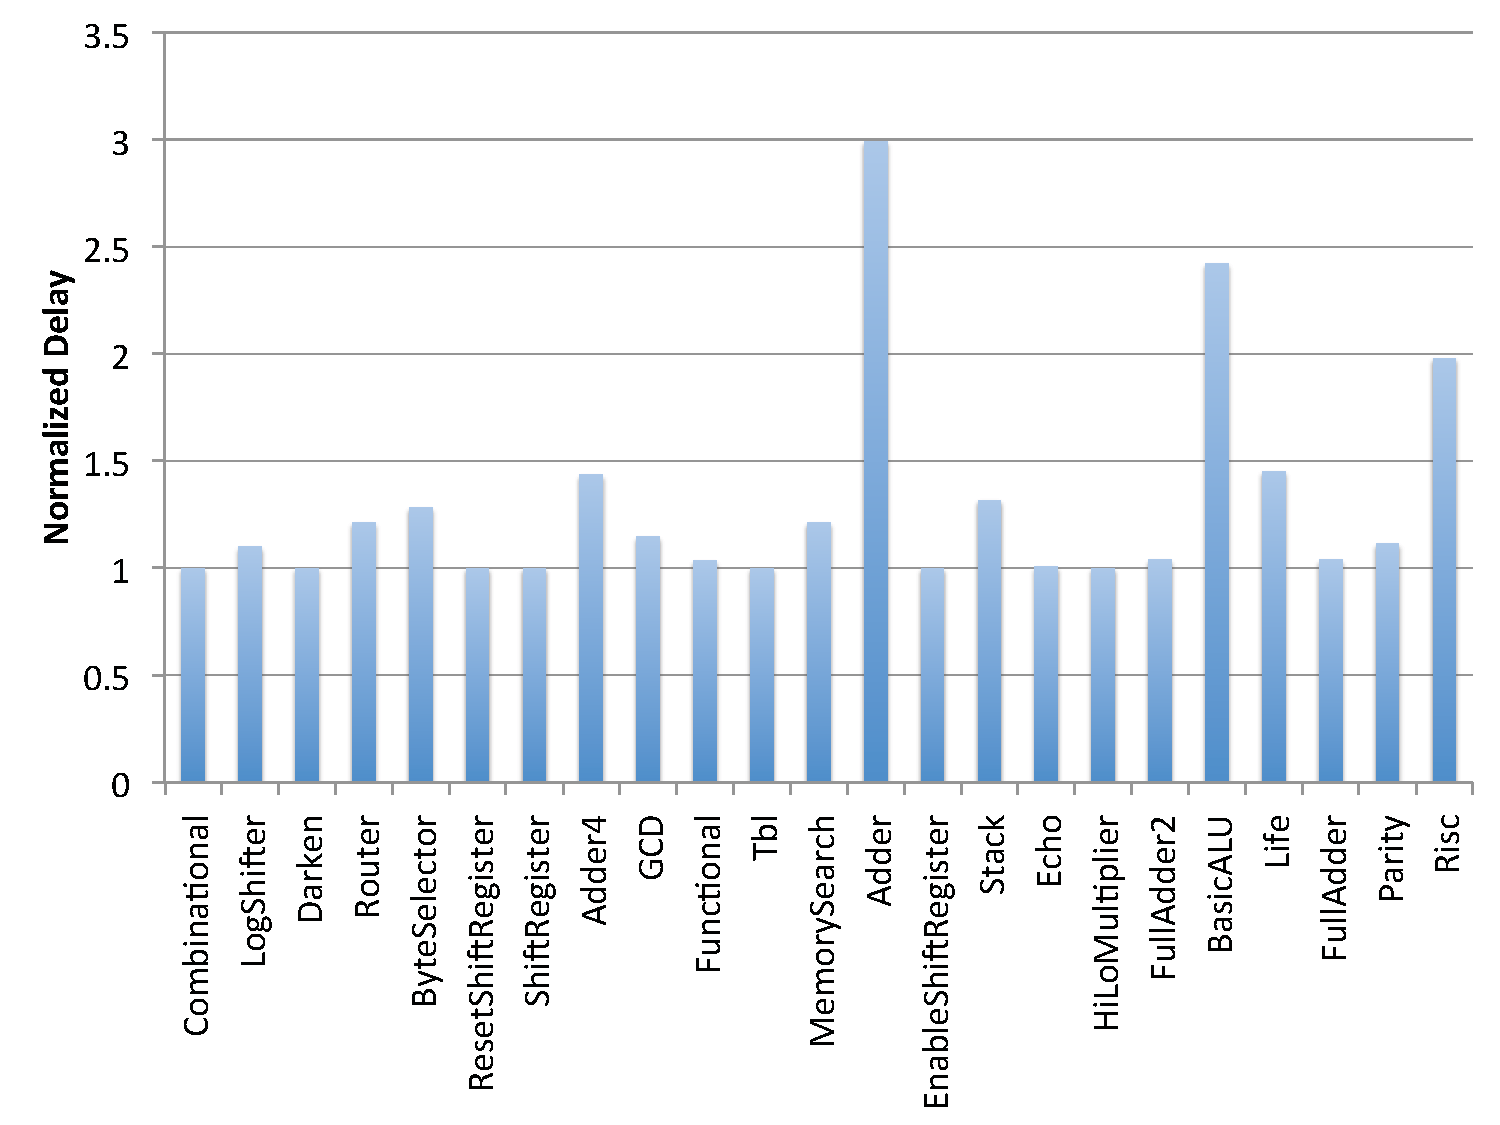
\includegraphics{figures/backannotation_result}}
    \caption{The critical path delays from the Chisel backannotator normalized to those from Design Compiler. We use example Chisel designs in the Chisel tutorial}
	\label{fig:backannotation_result}
\end{figure}
\subsection{Chisel Backannotation}
To verify the Chisel backannotator, we compare the critical path delays from the Chisel backannotator with those from Design Compiler. Figure \ref{fig:backannotation_result} shows the critical path delays calculated by the Chisel backannotator normalized to those calculated by Design Compiler. Design Compiler executes with minimal optimizations, which only checks hold time constraints. With the ideal Chisel backannotator, the normalized critical path delays should be equal to 1. The delays of most designs are very close to 1.

However, those of designs like Adder, BasicALU, and Risc are far away from 1. The inaccuracy of the backannotation mainly comes from the arrival time estimation for missing signals presented in Section \ref{sec:challenges}. It is possible for a Chisel node to have a delay number greater than its actual delay. For example, suppose there are only two timing paths P1 and P2 in the design. P1 is a path from X through T1, T2, and T3 to Y, and P2 is a path from X through T1 and T4 to Y where T1, T2, T3, and T4 are missing signals. We also assume that the delay of P1 is 4 and the delay of P2 is 3.9. In this case, the critical path is P1 whose delay is 4. The Chisel backannotator estimates the arrival times of T1, T2, T3 are 1, 2, 3, respectively, when reading the timing report of P1, while it estimates those of T1, T4 is 1.3, 2,6, respectively, when reading the timing report of P2. The Chisel backannotator concludes the delay of the node whose output signal is T1 or Y is 1.3 and the critical path delay is 4.6. This explains why some designs such as Adder, BasicALU, Risc, and Life have a normalized critical path delay much greater than 1.

To be worse, the fact that a design has a normalized delay equal to 1 does not mean each Chisel node has the exact delay number. This is because the arrival time of missing signals are estimated, which might not affect the critical path delay. For this reason, we need additional accuracy validation for the Chisel backannotator. 

\subsection{Automatic Pipeline Register Placement}
\label{auto_result}

\begin{table}[htb]
	\centering
	\resizebox{\columnwidth}{!}{
	\begin{tabular} 
		{ | l | r | r | r | }
		\hline
		& \textbf{Simple FSM} & \textbf{Simple RISC} & \textbf{Sodor} \\
		\hline \hline
		Number of Stages & $4$ & $4$ & $4$ \\
		\hline
		Max Unpipelined Combinational Path Delay & $125$ & $285$ & $380$ \\
		\hline
		Best Possible Pipelined Combinational Path Delay & $31.25$ & $71.25$ & $95$ \\
		\hline
		Actual Pipelined Combinational Path Delay & $50$ & $135$ & $175$ \\
		\hline
		Actual Pipelined Delay / Best Possible Pipelined Delay & $1.6$ & $1.89$ & $1.84$ \\
		\hline
	\end{tabular}
	}
	\caption{{\bf Pipelined Design Delay Data} The delays are obtained from analyzing the Chisel node graph pre synthesis. The delays are unitless because they are obtained from arbitrary mock delays assigned for the sake of independently testing the automatic pipeline placement tool}
	\label{fig:mock_delays}
\end{table}

%\begin{figure}[htb]
%\centering
%\resizebox{\columnwidth}{!}{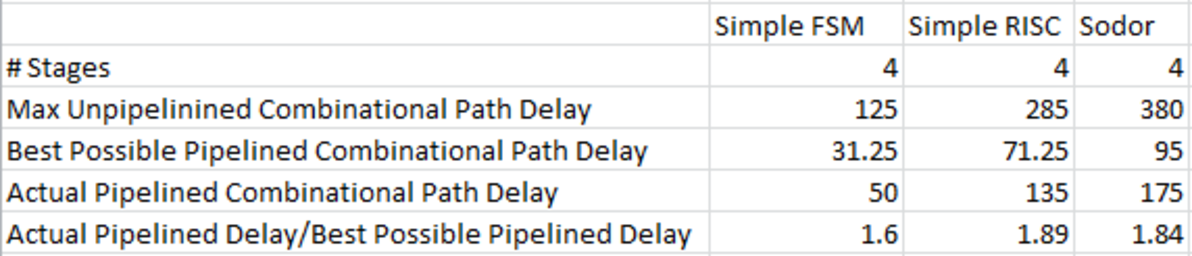
\includegraphics{figures/mock_delay_stats.pdf}}
%\caption{{\bf Pipelined Design Delay Data} The delays are unit less they are arbitrary units used for the sake of independently testing the automatic pipeline placement.}
%\label{fig:mock_delays}
%\end{figure}

We first want to evaluate the automatic pipeline placement independently from the Chisel Backannotation. Thus, we first run a very simple finite state machine, a simple RISC processor, and the Sodor processor through the automatic pipeline tools using mock delay numbers. Every Chisel Op node is give a mock delay of 5 and all other Chisel nodes are given mock delays of 0. Delay data is obtained by analysing the final Chisel graph after the automatic pipelining tool finishes placing the pipeline registers. For each example, we can obtain the best possible pipelined combinational path delay by dividing the maximum unpipelined combinational path delay by the number of pipeline stages. Then we can compare the actual pipelined combinational path delay against this best possible pipelined combinational path delay to get an idea of how well the automatic register placement is doing. We should not expect the tool to match the best possible pipelined combinational path delay because combinational logic nodes are not arbitrarily divisible and do not have uniform delays.

As seen in Table \ref{fig:mock_delays}, the automatic pipeline tool achieves relatively good  placement on a very simple finite state machine and slightly worse placement on the simple RISC processor ad the Sodor processor. This trend is explained by the fact that the automatic pipelining tool is more constrained on where it can place the pipeline registers on the more complex designs. Several things constrain the placement of the pipeline registers:

{\bf (1)} 
As discussed previously, the tool is not allowed to move IO nodes across pipeline stage boundaries. In more complex designs, there are more IO nodes and they prevent not only themselves, but also their inputs and consumers from being freely placed by the automatic pipelining tool. In the case of input nodes, its consumer nodes must be placed at a stage {\tt >=} the stage of the input node. In the case of output nodes, its input nodes must be placed at a stage {\tt <=} the stage of the output node.

{\bf (2)}  
The automatic pipelining tool cannot put pipeline registers in the middle of large black box modules such as caches. Thus, if the delay across the black box module is the critical path delay, the tool cannot reduce the critical path delay any further. The simple finite state machine does not use any black box modules while the more complex designs do.

{\bf (3)} 
The automatic pipelining tool cannot put pipeline registers between the input and output muxes of the read and write ports of array memories. In some designs, these read and write ports of array memories is a significant portion of the unpipelined critical path delay and thus the tool is unable to reduce the critical path delay below the propagation delay through the read and write ports of the array memories. The simple finite state machine does not use any array memories while the more complex designs each have an array memory for the register file.

Given these constraints, the automatic pipeline placement does a reasonable job placing the pipeline registers.
\subsection{Combined Tool Results}
\begin{table}[htb]
	\centering
	\resizebox{\columnwidth}{!}{
	\begin{tabular} 
		{ | l | r | r | r | }
		\hline
		& \textbf{Simple FSM} & \textbf{Simple RISC} \\
		\hline \hline
		Number of Stages & $2$ & $2$ \\
		\hline
		Max Unpipelined Combinational Path Delay & $0.9943$ & $0.5215$ \\
		\hline
		Best Possible Pipelined Combinational Path Delay & $0.49715$ & $0.26075$ \\
		\hline
		Actual Pipelined Combinational Path Delay & $0.5703$ & $0.5215$ \\
		\hline
		Actual Pipelined Delay / Best Possible Pipelined Delay & $1.15$ & $2$ \\
		\hline
	\end{tabular} }
	\caption{{\bf 2 Stage Pipelined Design Delay Data} The delays are in units of ns and are obtained from post-synthesis data.}
	\label{fig:comb_delays2}
\end{table}

\begin{table}[htb]	
	\resizebox{\columnwidth}{!}{
	\begin{tabular} 
		{ | l | r | r | r | }
		\hline
		& \textbf{Simple FSM} & \textbf{Simple RISC} \\
		\hline \hline
		Number of Stages & $3$ & $3$ \\
		\hline
		Max Unpipelined Combinational Path Delay & $0.9943$ & $0.5215$ \\
		\hline
		Best Possible Pipelined Combinational Path Delay & $0.3314$ & $0.1738$ \\
		\hline
		Actual Pipelined Combinational Path Delay & $0.418$ & $0.5215$ \\
		\hline
		Actual Pipelined Delay / Best Possible Pipelined Delay & $1.26$ & $3$ \\
		\hline
	\end{tabular} }
	\caption{{\bf 3 Stage Pipelined Design Delay Data} The delays are in units of ns and are obtained from post-synthesis data.}
	\label{fig:comb_delays3}	
\end{table}

\begin{table}[htb]	
	\resizebox{\columnwidth}{!}{
	\begin{tabular} 
		{ | l | r | r | r | }
		\hline
		& \textbf{Simple FSM} & \textbf{Simple RISC} \\
		\hline \hline
		Number of Stages & $2$ & $2$ \\
		\hline
		Max Unpipelined Combinational Path Delay & $0.9943$ & $0.5215$ \\
		\hline
		Best Possible Pipelined Combinational Path Delay & $0.248575$ & $0.130375$ \\
		\hline
		Actual Pipelined Combinational Path Delay & $0.418$ & $0.5215$ \\
		\hline
		Actual Pipelined Delay / Best Possible Pipelined Delay & $1.68$ & $4$ \\
		\hline
	\end{tabular} }
	\caption{{\bf 4 Stage Pipelined Design Delay Data} The delays are in units of ns and are obtained from post-synthesis data.}
	\label{fig:comb_delays4}	
\end{table}

%\begin{figure}[htb]
%\centering
%\resizebox{\columnwidth}{!}{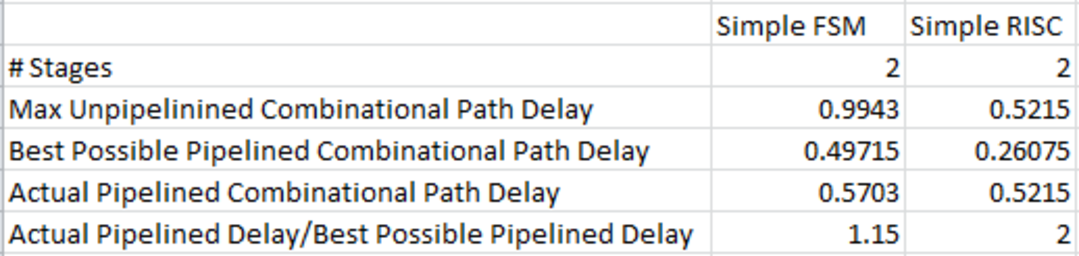
\includegraphics{figures/combined_delay_stats2.pdf}}
%\caption{{\bf 2 Stage Pipelined Design Delay Data} The delays are in units of ns.}
%\label{fig:comb_delays2}
%\end{figure}
%\begin{figure}[htb]
%\centering
%\resizebox{\columnwidth}{!}{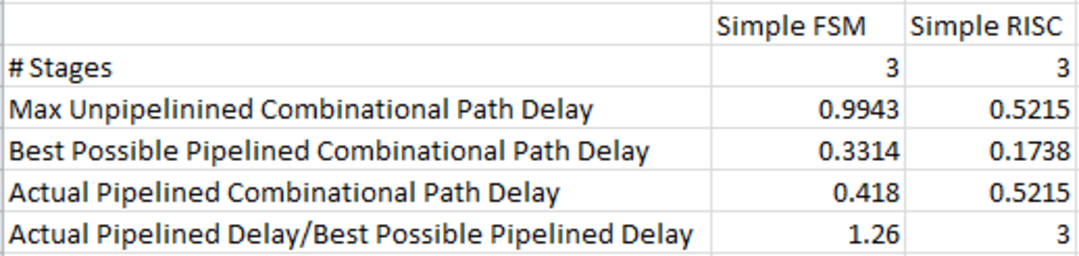
\includegraphics{figures/combined_delay_stats3.pdf}}
%\caption{{\bf 3 Stage Pipelined Design Delay Data} The delays are in units of ns.}
%\label{fig:comb_delays3}
%\end{figure}
%\begin{figure}[htb]
%\centering
%\resizebox{\columnwidth}{!}{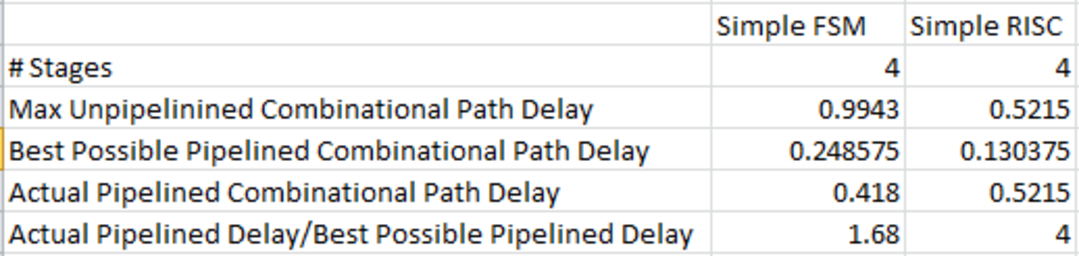
\includegraphics{figures/combined_delay_stats4.pdf}}
%\caption{{\bf 4 Stage Pipelined Design Delay Data} The delays are in units of ns.}
%\label{fig:comb_delays4}
%\end{figure}

We now evaluate the performance of the automatic pipeline performance when using real delay data obtained from Chisel backannotation with the same metrics as the above section. The delay data is obtained by running the simple finite state machine and the simple RISC processor through the full combined tool flow involving the backannotation, the automatic pipelining, and finally synthesis. Synthesis is run with gate level optimizations turned off because we want to try to preserve a one to one mapping between the gate netlist and the Chisel node graph. We do not use the Sodor processors in the evaluation because we are unable to obtain delay data from them as they contain very large unsynthesizable scratchpad memories. We do not use post-place and route data because they introduce extra noise into the delay data due to how non-predictable layout patterns affect wire delays.

Table \ref{fig:comb_delays2}, Table \ref{fig:comb_delays3}, and Table \ref{fig:comb_delays4} show that the automatic pipelining tool performs very well on 2, 3, and 4 stage versions of the simple finite state machine, with actual pipelined combinational path delays being very close to best possible pipelined combinational delays.  This shows that given a sufficiently unconstrained design, automatic pipeline placement is able to do a good job when integrated with the real delay data provided by Chisel backannotation.

Table \ref{fig:comb_delays2}, Table \ref{fig:comb_delays3}, and Table \ref{fig:comb_delays4} show that the automatic pipelining tool performs very poorly for the simple RISC processor. In fact, the critical path delay is the same for the 2,3, and 4 stage versions of the design. This is caused by constraint (3) described in \ref{auto_result}. In this case the critical path of the simple RISC processor is dominated by the muxes in the read port of its register file. The automatic pipelining tool has no way to place pipeline registers between these muxes, so the critical path delay is identical for the 2,3, and 4 stage designs.

